% Created 2024-04-22 Mon 19:37
% Intended LaTeX compiler: pdflatex
\documentclass[letterpaper, 10pt, twocolumn]{article}
                      \usepackage{lmodern} % Ensures we have the right font
\usepackage[T1]{fontenc}
\usepackage[utf8]{inputenc}
\usepackage{graphicx}
\usepackage{amsmath, amsthm, amssymb}
\usepackage[table, xcdraw]{xcolor}
\renewcommand{\thesection}{\Roman{section}}
\renewcommand{\thesubsection}{}
\renewcommand{\thesubsubsection}{}
\definecolor{bblue}{HTML}{0645AD}
\usepackage[colorlinks]{hyperref}
\hypersetup{colorlinks, linkcolor=blue, urlcolor=bblue}
\usepackage{titling}
\setlength{\droptitle}{-6em}
\setlength{\parindent}{12pt}
\setlength{\parskip}{0em}
\usepackage[stretch=10]{microtype}
\usepackage{hyphenat}
\usepackage{ragged2e}
\usepackage{subfig} % Subfigures (not needed in Org I think)
\usepackage{hyperref} % Links
\usepackage{listings} % Code highlighting
\usepackage[top=1in, bottom=1.00in, left=0.85in, right=0.85in]{geometry}
\renewcommand{\baselinestretch}{1.00}
\usepackage[explicit]{titlesec}
\pretitle{\begin{center}\fontsize{20pt}{20pt}\selectfont}
\posttitle{\par\end{center}}
\preauthor{\begin{center}\vspace{-6bp}\fontsize{12pt}{12pt}\selectfont}
\postauthor{\par\end{center}\vspace{-25bp}}
\predate{\begin{center}\fontsize{12pt}{12pt}\selectfont\vspace{1em}}
\postdate{\par\end{center}\vspace{0em}}
\titlespacing\section{0pt}{5pt}{5pt} % left margin, space before section header, space after section header
\titlespacing\subsection{0pt}{5pt}{2pt} % left margin, space before subsection header, space after subsection header
\titlespacing\subsubsection{0pt}{5pt}{-2pt} % left margin, space before subsection header, space after subsection header
\usepackage{enumitem}
\setlist{itemsep=-2pt} % or \setlist{noitemsep} to leave space around whole list
\usepackage{listings}
\author{jmowry4@vols.utk.edu}
\date{4/16/24}
\title{\textbf{Maximizing Requests per Second on a Single Thread through \texttt{io\_uring}}\\\medskip
\large Jackson Mowry}
\hypersetup{
 pdfauthor={jmowry4@vols.utk.edu},
 pdftitle={\textbf{Maximizing Requests per Second on a Single Thread through \texttt{io\_uring}}},
 pdfkeywords={},
 pdfsubject={},
 pdfcreator={Emacs 29.3 (Org mode 9.7)}, 
 pdflang={English}}
\begin{document}

\maketitle
\section{Abstract}
\label{sec:orgb831e27}
\textbf{This research paper investigates the transformative potential of io\textsubscript{uring} in scaling HTTP web servers to accommodate the needs of numerous concurrent clients. Despite the extensive exploration of various scaling techniques, little attention has been paid to the potential paradigm shift that \texttt{io\_uring} may introduce in asynchronous I/O architectures. \texttt{io\_uring} enables the handling of workloads traditionally confined to highly parallelized systems. This paper aims to explore the implications of \texttt{io\_uring} on asynchronous I/O systems, shedding light on its promise for enhancing server scalability and performance in the face of ever increasing demands.}
\section{Introduction}
\label{sec:org0ae2fcd}
Web servers are a piece of software that sit between nearly every interaction a client makes on their device, and access to the files housed on a server. Despite this fact they are rarely inovated on, due to the fact that for most use cases they are ``good enough''. It is true that even a naive HTTP server can serve thousands of requests per second, which easily surpasses the needs of most users. The same architecture can be transplanted on top of a machine with many CPU cores in order to scale up to meet demands.

But these workloads are still inhrently synchronous at some level (excluding \texttt{aio}). \texttt{io\_uring} brings a true asynchronous io system to the table with its introduction into the Linux kernel (version 5.1).

In this article we will explore ``\href{https://wiki.c2.com/?IoMultiplexing}{multiplexed io}'' on linux through the use of \texttt{io\_uring}. Implementations are compared to the best possible implementation on a single core under other programming models. Along with single core tests we will pit our single core against a threaded server.
\section{Previous Work}
\label{sec:org08ee608}
\subsection{{\bfseries\sffamily TODO} }
\label{sec:org56dfc76}
\section{Asynchronous IO}
\label{sec:org1d11468}
Most if not all system calls used in day to day software are considered ``blocking'', meaning they will only return once the entire function has finished executing. This model allows for programs to not having to worry about order of execution, as they know their program will run top to bottom without skipping a step. However, large web servers simply cannot afford to spend the time waiting for each system call to execute to completion. To avoid this problem of blocking programmers may choose to design their software around asynchronous IO.

On Linux this has taken the form of \texttt{epoll}, which allows for certain operations to be performed without blocking the main thread of execution.
\section{\texttt{aio}}
\label{sec:org20dd43e}
The \texttt{aio} system in Linux has two implementations, POSIX compliant, and the Linux implementation. Both systems suffer the same issue, they are intended to work with regular files, and as such don't play well with sockets. glibc creates a thread pool to perform regular synchronous io off the main thread, giving the illusion of asynchronosity.

For all of these reasons \texttt{aio} is generally avoided in application code.
\section{\texttt{epoll}}
\label{sec:org2a4fe44}
\texttt{epoll} is kernel based implementation of \texttt{poll}, with both providing a way to monitor a range of file descriptors, and alerting the user when one or many are ready for IO. It has become a very common architecture for web servers and other asychronous io systems to be built on top of. Most notably to implement the primatives golang's \texttt{net/http} package is built upon, and \texttt{libuv} which powers the Node.js event loop.

\texttt{epoll} expands on the original ideas of poll by sharing a list of file descriptors between the user and kernel, preventing the need for data to be copied back and forth. When any number of file descriptors are ready for IO they will be placed in a separate shared list, which the user can then perform the desired action on.

This architecture allows for a single thread to handle large numbers of active file descriptors, only slowing down to perform the synchronous operations like reading or writing. The actual implementation does not allow for asynchronous sending or recieving of data, merely alerting the user when those operations can be performed without blocking.

One downside of \texttt{epoll} is that it does not behave consistently across file descriptors of different types. While it is true that recieving data from a socket can block, which \texttt{epoll} is aware of, regular files do not exhibit the same behavior. On Linux read and write calls to a file should not block, but as we all know this is not true. You can make a write call and expect it to complete instantly, but if the kernels write cache is full, you will have to wait. The same goes for a read call which can blocked if the file is on a slow drive.
\section{\texttt{io\_uring}}
\label{sec:org113b28f}
\texttt{io\_uring} is the latest attempt at adding asynchronous operations to Linux. Its design makes it obvious that it the designer learned from many of the shortcomings of \texttt{aio}. Not only does \texttt{io\_uring} provide a common interface across all types of file descriptors, it also implements most systems calls in an asyncronous fashion.

The design can be broken down into two distinct parts, a job submission queue, and a job completion queue, both implemented via ring buffers shared between the kernel and user space. At a basic level each submission is a combination of an op code defining which system call to perform, and the associated arguments. If the user desires to keep track of a job they can associate user data with a submission, which takes the form of an 64-bit integer, commonly used to hold a pointer. The implementation garuntees that user data will not be modified.

Once a job is complete it is placed in the completion queue, which an application can pull from. Completions have 2 main fields to pay attention to: a result code, and the associated user data. The result code is analogous to the return value from regular blocking system calls with one exception. Due to the concurrent execution of submissions the system cannot garuntee that the \texttt{ERRNO} associated with each system call will still be properly set when a user recieves a completion. Instead, \texttt{ERRNO} is placed in the completion struct, with its value negated so that it will not be confused with a successful execution.

\texttt{io\_uring} also offers one distinct advantage over the other asynchronous io methods presented here. Jobs can be submitted through a system call, or by having the kernel continuously poll the submission queue using a separate thread. This allows for a program to operate entirely in user space, avoiding system calls which have become even more costly in the age of speculative execution mitigations. We will explore both methods of job submission to see where their advantages lie.

Being the latest in the asyncronous IO space \texttt{io\_uring} is still lacking some features. Most notably is missing system calls, and event notification on a submission/completion level. Most missing system calls can be implemented without changing the underlying system, with the remaining few not being necessary to implement asynchronously.
\section{System Calls}
\label{sec:org67487a4}
One of the major mitigations put into place after the speculative execution attacks were discovered (spectr and meltdown) was isolation of kernel and user space memory. This slows system calls as they now have to switch into a different address space to perform the operation, and switch back once they're done.

To mitigate this modern software systems have transitioned to a model where system calls are avoided, sometimes entirely. The most obvious implementations of this are systems that manage memory allocations themselves, or those that manage files using shared memory.

\texttt{io\_uring} allows the program to avoid system calls upon submission, meaning that a system can work entirely in userspace, without the need for costly system calls. This reduces the number of system calls from at a minimum 4 (accept, read, write, close) in a synchronous server, to a potential 0 in an \texttt{io\_uring} based approach.

Allowing system calls to proceed asynchronously also allows for a program to handle clients with heavy requests without blocking clients with lighter weight requests. This is a major advantage over synchronous servers where either an entire program is blocking reading/writing a file, or a thread is held up waiting. This can slow the overall throughput of these systems, whereas an asynchronous implementation would proceed handling other clients while a file is being read.
\section{Methods}
\label{sec:org7222102}
Testing will include an \texttt{epoll} server, four distinct \texttt{io\_uring} servers, and a sixth synchronous server using \texttt{poll}. Servers will parse a request, open a file, respond with the appropriate headers, send the file, and finally close the connection. Performance testing using \texttt{wrk} at \{1, 4, 8, 16, 32, 64, 128, 256, 512, 1024, 2048, 4096, 8192\} concurrent connections run over 30 seconds, with the mean of 3 runs reported for each metric.

For testing four \texttt{io\_uring} based servers will be compared. For a more realistic web server example only the accept, read, and close system calls will be replaced with their asynchronous counterparts, with the rest of the work handled synchronously. The other \texttt{io\_uring} server will replace every system call (except for \texttt{pipe} which does not yet exist) with their asynchronous versions. Each of these servers will also have submission queue polling enabled as an additional observation point.
\section{Results}
\label{sec:org2d4adac}
\begin{center}
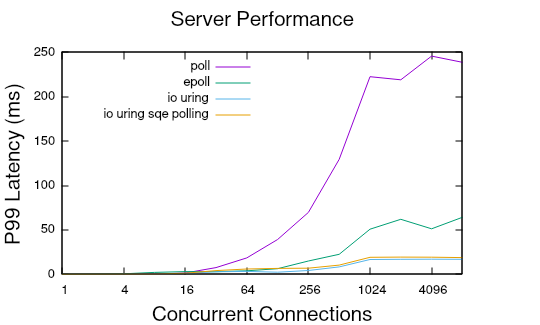
\includegraphics[width=10cm]{./p99_latency.png}
\end{center}

Each server was tested over all 13 connection loads in one pass. P99 latency is an important metric when analyzing the performance of any service, it indicates how the slowest 1\% of request are handled. As expected, the synchronous \texttt{poll} based server experiences substantial growth in latency as the number of concurrent request in increased. This is due to the fact the scanning the list of watched file descriptors happens in linear time as each is checked for a \texttt{POLLIN} event. The \texttt{epoll} server is able to maintain a similar latency to either \texttt{io\_uring} server until 128 concurrent request when it begins to climb rapidly. Latency continues to grow with connections, and would be expected to continue rising.

Both \texttt{io\_uring} servers exhibit similar P99 latency, quickly reaching a plateau around 25ms from 1024 concurrent requests and beyond. One of the key benefits of \texttt{io\_uring} is its ability to handle massively concurrent workloads, as observed with either implementation. Submission queue polling increases latency by a fixed amount across the entire test range due to the separate kernel thread which must watch the queue. However, the slower latency values are potentially a worthwile tradeoff for some applications where the ability to avoid system calls all together is necessary.

\begin{center}
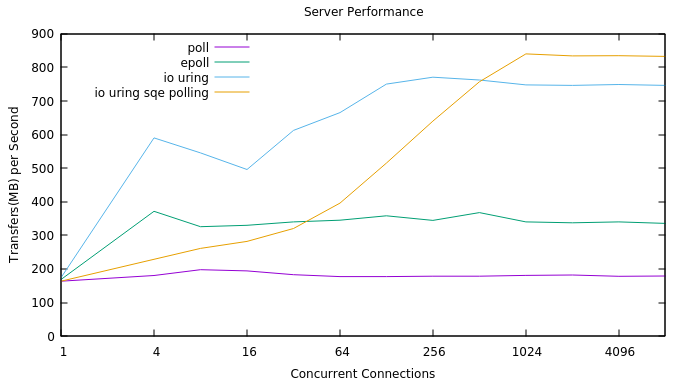
\includegraphics[width=.9\linewidth]{mbps.pn.png}
\end{center}
\begin{center}
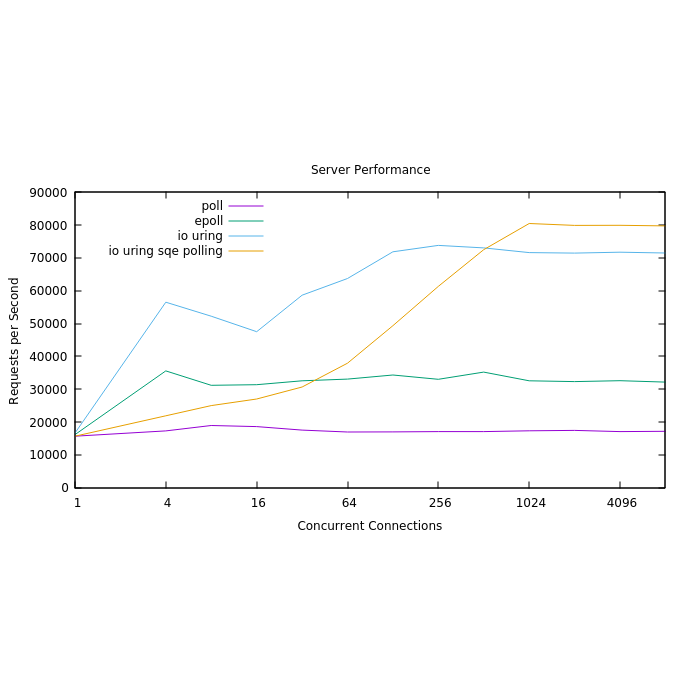
\includegraphics[width=.9\linewidth]{rps.png}
\end{center}

Throughput of the synchronous server follows our expectations, a nearly flat line across the entire testing range. The rate at which we can push data over the wire is entirely limited by the fact that each request is handled one at a time, which is entirely dependent on the time on which we are blocked in system calls. For simple applications this approach may be enough to handle the workload, and it comes with the upside that a \texttt{poll} implementation is a much simpler architecture.

\texttt{epoll} exhibits nearly the same behavior as the poll based implementation, only at a higher overall throughput. We see no degradation in performace for either server up to 8192 concurrent request. The advantage for \texttt{epoll} comes in the fact that it's ``work queue'' is only populated with requests that have data ready, meaning that each file descriptor can have work done without having to check its status.

A basic \texttt{io\_uring} server without submission queue polling quickly reaches its maximum throughput at 128 concurrent requests, which the server is able to maintain all the way up through 8192 concurrent requests. This equates to a maximum throughput of around 750MB/s, or \textasciitilde{}6Gbit/s, serving a 12KB text file to each client. When submission queue polling is enabled we see an interesting shift in throughput. A much lower throughput is seen at lower concurrent requests, which quickly jumps past the original implementation at 512 concurrent requests. From 512 requests and beyond a gap of just under 10,000 requests per second is maintained. This equated to a gap of around 100MB/s, or 0.8Gbit/s.
\section{Discussion}
\label{sec:org0d6e467}
Either asynchronous implementation offers obvious advantages over an entirely synchronous server. \texttt{epoll} offers an interesting middle ground where the architecture is simpler, at the cost of reduced throughput. However, \texttt{epoll} has better portability when if the application needs to run on the family UNIX based systems. Linux has \texttt{epoll}, while MacOS and BSD both have \texttt{kqueue}, which offers a similar API for performing asynchronous operations on file descriptors. \texttt{epoll} has also been around since Linux kernel version 2.5 (2002), meaning resources and documentation are more widely available.

As discussed before, one potential disadvantage with \texttt{epoll} is that it only works well with sockets, or files opened in an unbuffered/direct mode. If an application needs to do more than accept an incoming connection on a socket and send back a response, \texttt{epoll} will not be useful for other operations.

\texttt{io\_uring} has shown that with its superior implementation it can out perform the contemporary way we build web servers. Showing a 75.95\% improvement (85.01\% for SQ polling) in throughput over the \texttt{epoll} based server at 8192 concurrent requests. The worst case latency of an \texttt{io\_uring} server also scales better than \texttt{epoll}, exhibiting 1/4 the latency at 8192 concurrent requests.
\section{Cite}
\label{sec:org5472c40}
\url{https://www.kernel.org/doc/ols/2003/ols2003-pages-351-366.pdf}
\url{https://www.landley.net/kdocs/mirror/ols2004v1.pdf\#page=215}
\url{https://darkcoding.net/software/linux-what-can-you-epoll/}
\url{https://darkcoding.net/software/epoll-the-api-that-powers-the-modern-internet/}
\end{document}
